\chapter{The \LHC and the \CMS experiment}
\label{chap:detector}

%\chapterquote{There, sir! that is the perfection of vessels!}
%{Jules Verne, 1828--1905}
The purpose of this chapter is to introduce the \CMS experiment and the \LHC \cite{1748-0221-3-08-S08001}. Without both of these apparatus the analyses performed for this thesis would, of course, not have been possible. In \SectionRef{sec:lhc} an overview of the \LHC and the chain of accelerators which feed into it will be given. This will then be followed in section \SectionRef{sec:CMSIndetail} by a description of the \CMS experiment focussing on the aspects most relevant to the search for invisibly decaying Higgs bosons.

\section{The \LHC}
\label{sec:lhc}
The \LHC is situated 100m underground in a tunnel formerly built for the LEP accelerator~\cite{lepdesign} at CERN near Geneva, Switzerland. It is a 27km storage ring which accelerates both protons and heavy ions and collides them at the highest centre of mass energies of any collider built to date. The work contained in this thesis uses data from proton-proton collisions. These protons are obtained by taking hydrogen gas and stripping its atoms of their electrons with an electric field. The first accelerator in the \LHC accelerator sequence, Linac 2, then accelerates the protons to 50 \MeV. The protons are then accelerated to 1.4 \GeV by the next accelerator, the Proton Synchrotron Booster (PSB), which is followed by the Proton Synchrotron (PS) where they reach 25 \GeV. The beam energy is then increased to 450 \GeV in the Super Proton Synchrotron (SPS). The protons are then injected into the \LHC where, at time of writing, the maximum energy the beams have been accelerated to is 6.5 \TeV, close to its design maximum of 7 \TeV.

When fully filled the \LHC contains two counter-rotating beams which are formed of up to 2808 bunches spaced either 25 or 50 ns apart and each containing $\mathcal{O}(10^{11})$ protons. The two beams are kept travelling in a cirlce by 1232 superconducting dipole magnets and steered to four collision points around the \LHC. Detectors are situated at these collision points to observe the collisions, the main four being: ALICE~\cite{Aamodt:2008zz}, ATLAS~\cite{Aad:1129811}, CMS~\cite{Chatrchyan:2008aa} and LHCb~\cite{Alves:2008zz}. A schematic of the LHC accelerator chain and the detectors can be seen in \FigureRef{fig:lhclayout}

\begin{figure}
  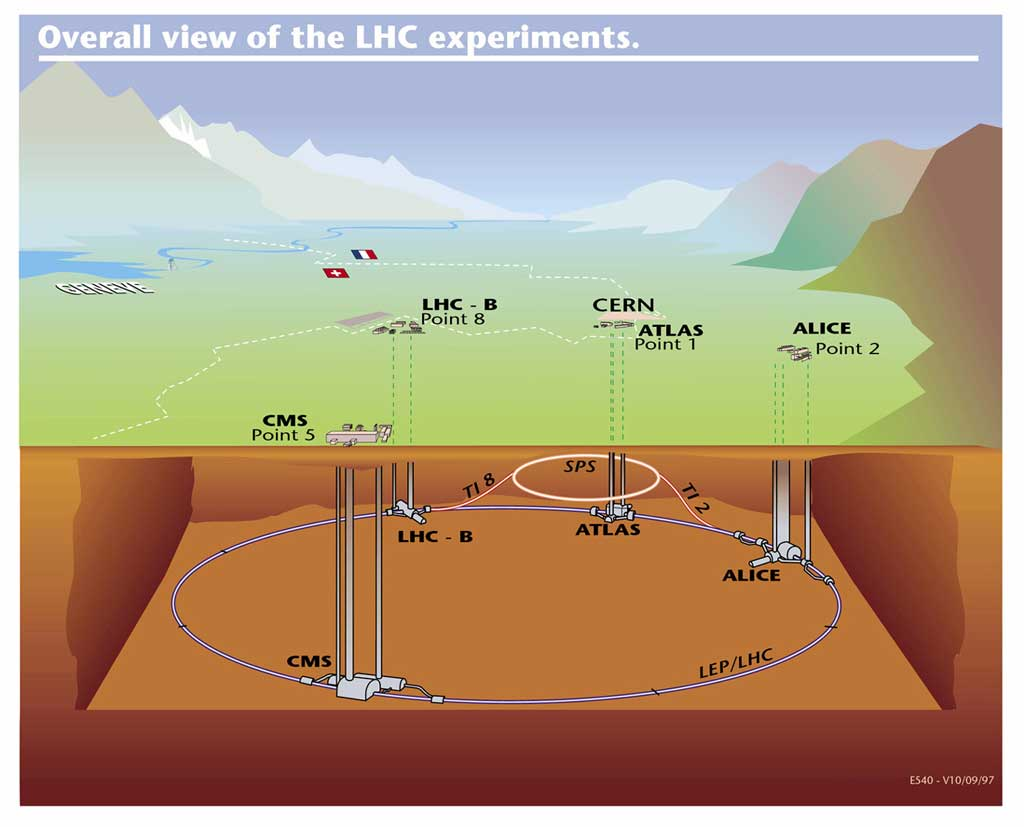
\includegraphics[width=\largefigwidth]{plots/detector/lhc_layout_sch.jpg}
  \caption{A schematic of the LHC accelerator and the positions of the four main detectors.}
  \label{fig:lhclayout}
\end{figure}

%!!IMAGE OF ACCELERATOR COMPLEX

%!!Discuss luminosity and why it needs to be so high for Higgs
%!!Discuss operation at energies
%!!Discuss pileup

\section{The \CMS experiment}
\label{sec:CMSInDetail}


\subsection{Trigger system}
\label{sec:triggers}


